\graphicspath{{./figures/}}
\chapter{Methodology} 
The following chapter provides an overview over the relevant development 
components that are used within this project.
Therefore, the used software packages are introduced before a short outline of
the utilized drone hardware is given.

\section{Software fundamentals}\label{sec:2_software_fund}
As the main part of this project's software will run on a portable remote
computer allowing for not only to control the drone but also for performing the
long jump analysis on video inputs, every software component is chosen to
demand as little hardware requirements as possible.
Especially no \ac{GPU} is required to run the software.
All image processing is performed using the \ac{CPU} only.
Furthermore, the software is designed to run platform independent.\\

\subsection{Programming Language and why Python}\label{subsec:2_programming_language}
Because of its interpreted nature and many cross-platform libraries, Python is
one of the most used programming languages in the scientific area.
Furthermore, it offers a high level of abstraction allowing for rapid 
prototyping approaches which is a key factor for this project.
Besides fast implementation, Python nevertheless supports complex programming 
concepts like object-orientation.\\
Additionally, as stated in \autoref{subsec:2_mediapipe_framework} many machine
learning and \ac{AI} projects for detecting body poses have already been 
successfully implemented using Python.\\
Third party libraries and frameworks like \textit{OpenCV} for image processing 
and \textit{PyQt} for \ac{GUI} development are widely used and therefore well documented.
This leads to the decision to use Python as programming language within this work. 

\subsection{Mediapipe for detecting body poses}\label{subsec:2_mediapipe_framework}
One of the software's main tasks is to perform a human body pose detection on
video inputs.
Because this part runs on the remote computer only, it can also handle
pre-recorded videos that should be evaluated.\\
The evaluation itself is performed using the Mediapipe framework.
This framework uses a pre-trained convolutional neural network that is able to
detect 33 key points in human body poses \cite{mediapipe_paper}.
The network could theoretically even be fine-tuned to improve its accuracy on
specific input types.
Even if this so called \textit{transfer-training} method requires significantly
less training data compared to training a neural network from scratch, it is 
not applied within this project as first test runs already showed reliable 
results.\\
Furthermore, the Mediapipe framework does not require any hardware acceleration
and is renowned for its precise output.
Hii et al.~for example showed in~\cite{mp_gait_analysis}, 
\cite{mp_gait_analysis_2} that the framework can be applied in medical gait 
analysis applications to replace marker based approaches.\\
Moreover, Mediapipe offers three different detection models that differ in 
terms of speed and accuracy.
The fastest detection model offers the lowest accuracy and vice versa.\\
Additionally, Mediapipe is optimized for multiple input types including videos 
and live streams, which is ideal for this project.\\
\autoref{fig:2_body_keypoints} shows an overview of the 33 detectable key 
points. 
\begin{figure}[!h]
    \centering
    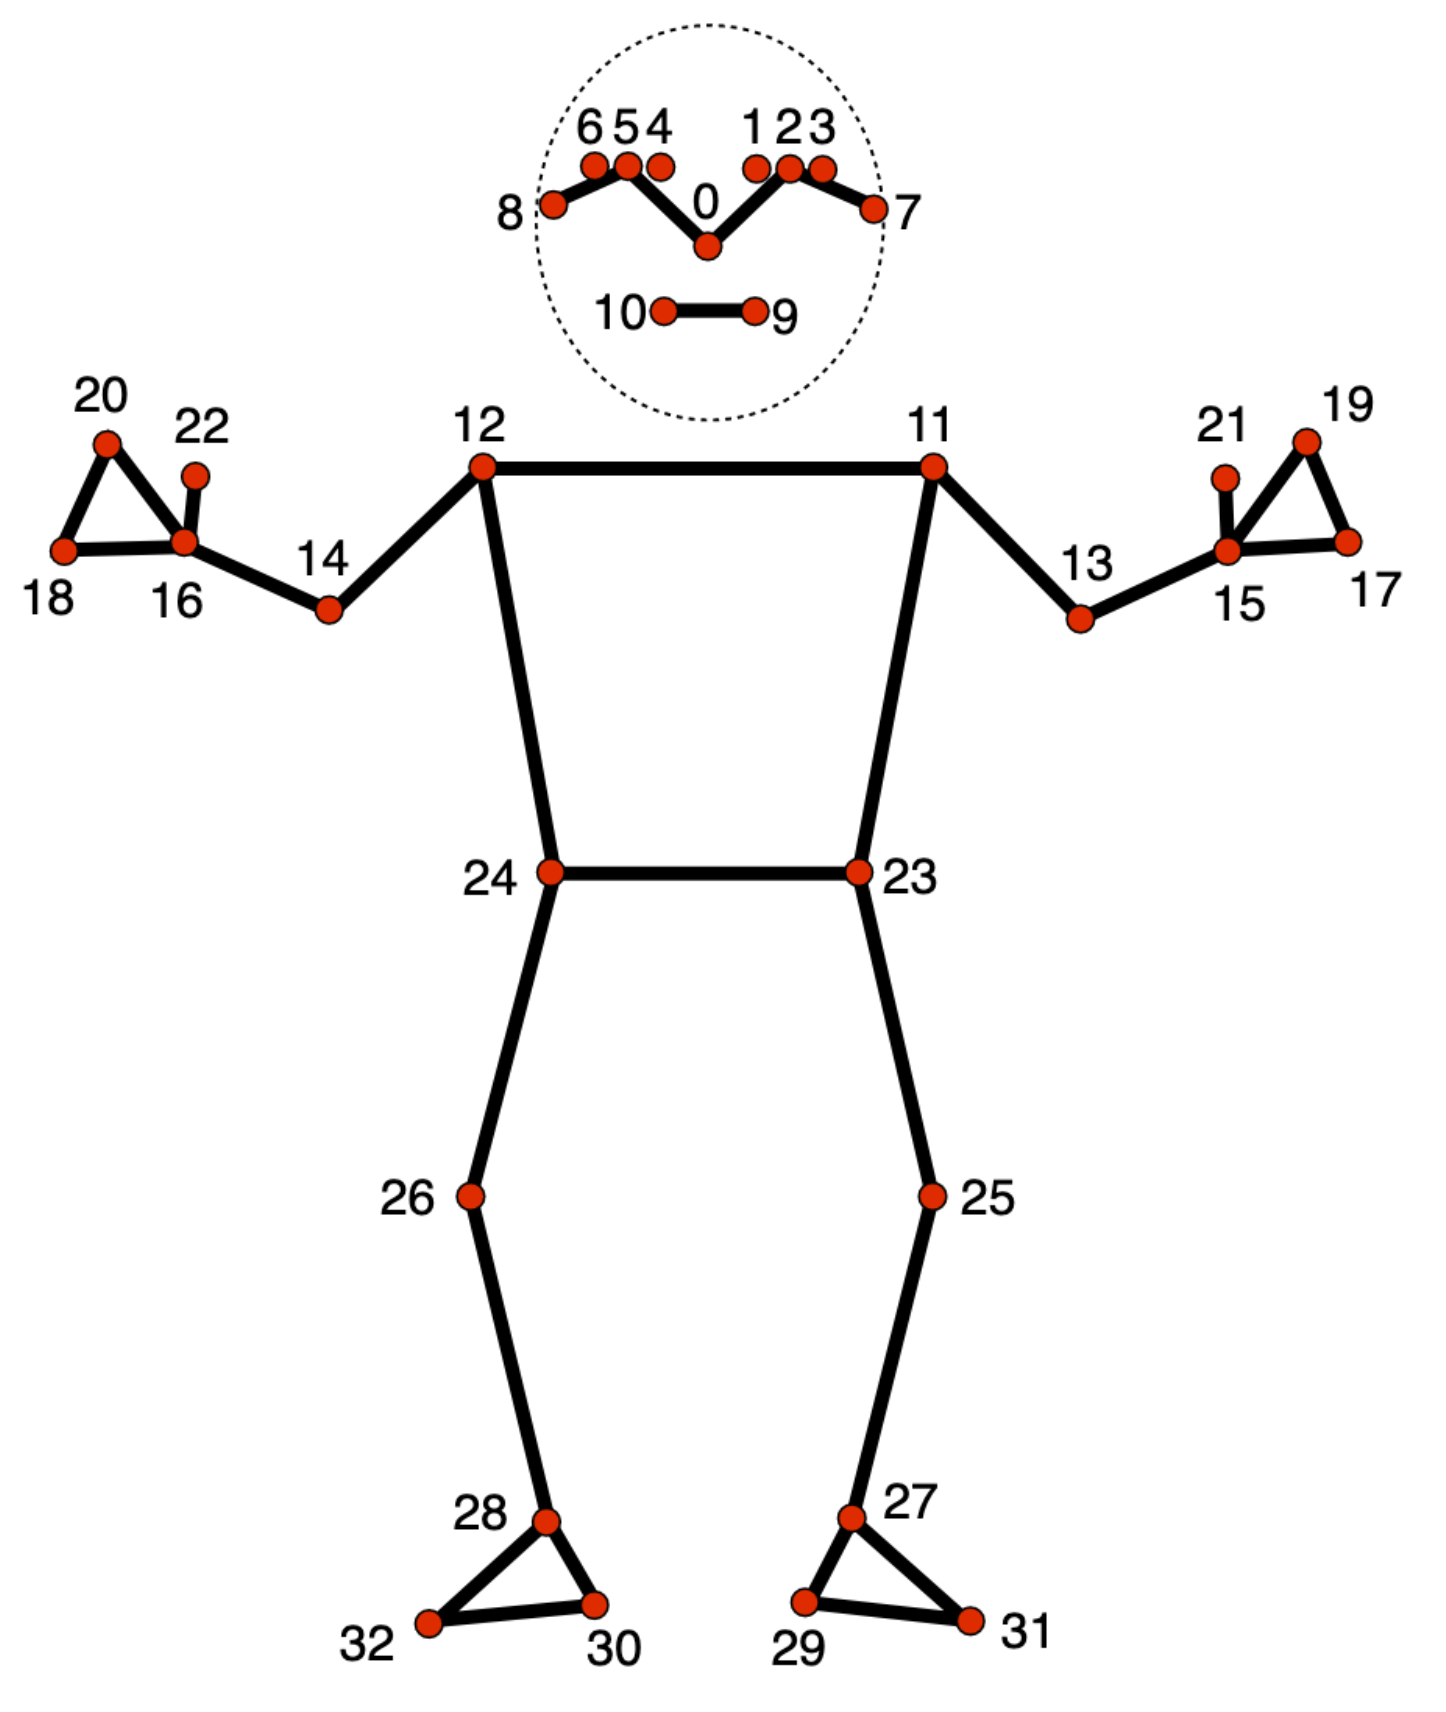
\includegraphics[scale=0.3]{figures/body_key_points.png}
    \caption[Set of detectable body key points]
    {Fixed set of detectable body key points offered by the mediapipe framework
    \cite{mediapipe_framework}}
    \label{fig:2_body_keypoints}
\end{figure}\\
Within this work, the key points in the head area (range [0 - 10]) are not of 
great interest apart from visualization purposes.\\
The knee, hip and arm key points however will be used for angle 
calculations and ground contact detection.
Thus, a good performance in detecting the according key points within these 
areas is crucial for the software's overall reliability.

\subsection{Why Mediapipe?}\label{subsec:2_why_mediapipe}
In recent years many approaches towards accurate body pose detection were 
developed and implemented.
Many of those offer decent accuracies, but often lack reasonable performance,
especially when no \ac{GPU} is available for hardware acceleration.
Following, two common alternatives to Mediapipe, namely OpenPose and AlphaPose,
are shortly presented and differentiated from the chosen Mediapipe framework.\\
One of the most widely used human pose detection libraries is the open source 
library \textit{OpenPose}.
As shown in~\cite{openPose} it offers a Multi-Person pose estimation that is 
especially useful when dealing with groups of people.
However, as this project is meant to be used for long jump evaluation, only one 
person needs to be tracked at a time.
Even though OpenPose of course can handle one person pose estimation, 
mediapipe outperforms OpenPose in this area.
Back in 2016 Kocabas et al.~achieved around 23~FPS using \ac{GPU} accelerated
OpenPose pose detection~\cite{openPose_speed_gpu} and Osokin later proposed an
improved neural network design, allowing for up to 28~FPS without hardware 
acceleration~\cite{openPose_speed_cpu}.
As of 2023 these benchmarks are still reasonable.
Mediapipe however achieves speeds of up to 63\% higher.\\
While OpenPose uses a \textit{Bottom-Up} approach due its multi-person 
application, Mediapipe uses the less computational complex \textit{Top-Down} 
approach.\\
Bottom-Up implementations first detect all body key points present in an input
image and then move on to grouping the recognized points in clusters.
Points in the same cluster are then assigned to one person.\\
Top-Down approaches however first roughly detect the overall body position 
within the input image and then define a region of interest\footnote{sometimes
also referred to as \textit{Bounding Box}} around the subject.
The following processing therefore only needs to take this defined region of 
interest into account, leading to significantly less computational complexity.\\
AlphaPose is another open source library often used for body pose estimation.
Just like OpenPose it uses a Bottom-Up approach to reliable offer multi-person
body pose detection.
Additionally, AlphaPose, like Mediapipe, offers multiple detection models that 
differ regarding accuracy and speed.
Again however, Mediapipe outperforms AlphaPose because of its Top-Down approach
and because AlphaPose is designed to work with \ac{GPU} acceleration, rather 
than running on \ac{CPU} only.\\
Another advantage of Mediapipe is its output.
While OpenPose and AlphaPose offer 2D coordinates for each detected key point,
Mediapipe additionally offers a depth estimation resulting in a spatial 3D 
coordinate for each detected key point.
Thereby, more comprehensive analysis can be performed.   

\subsection{OpenCV}\label{subsec:2_openCV}
OpenCV is an open source library commonly used for image processing in the 
area of computer vision and machine learning.
It is written in C++, thus offering high performance in numerical operations,
especially matrix operations.\\
\texttt{python-opencv} is the python wrapper for OpenCV which will be used in
this project to efficiently read and process video frames.
The python wrapper imports the underlying C++ functions as modules to take 
advantage of C++'s efficiency, resulting in significantly higher performance
compared to equivalent Python only implementations.
Furthermore, it is fully compatible with the \texttt{numpy} library, which 
allows for seamless conversion between numpy arrays and OpenCV image matrices.

\subsection{HDF5 file format}\label{subsec:2_hdf5}
To avoid analyzing the same jump, therefore the same video file, multiple 
times, the jump parameters should be saved after the analysis process alongside
with the annotated video file, that visualizes the detected body pose (see
\autoref{fig:2_body_keypoints}).
Because parameters such as knee angles, arm angles, ground contact, etc.\ need 
to be stored frame-wise, a structured file format is suitable.\\
One common open source structured file format is HDF5.
It is an acronym for Hierarchical Data Format (Version 5) and is very helpful 
to store large amounts of data as well as heterogeneous data. 
As the name already suggests, data is stored in a hierarchical, tree-like way.\\
A HDF5 tree mainly consists of three pre-defined components that allow to 
organize data in a file-system like fashion.
The tree root, groups and datasets.
\textit{Groups} are folder-like structures that can either contain more groups 
or Datasets.
\textit{Datasets} hold the actual data that need to be stored.\\
Furthermore, each level (tree root, groups and datasets) can hold additional 
information via metadata.
The metadata could for example contain information about metrics, timestamps or 
any other describing information.
Therefore, each HDF5 file itself becomes a self-describing file that does not
require any more than the included information to be interpreted correctly.\\
\begin{figure}[!h]
    \centering
    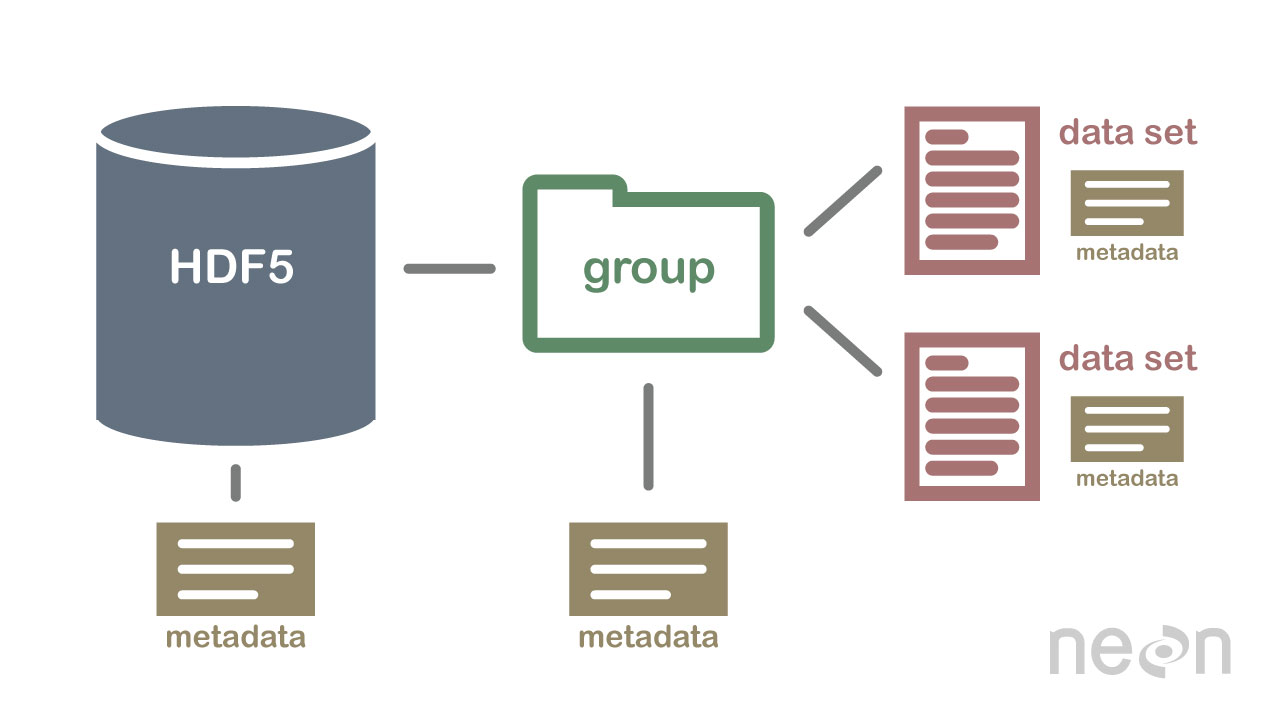
\includegraphics[scale=0.24]{figures/hdf5_general_structure.jpg}
    \caption[HDF5 file structure]
    {Principle HDF5 file structure~\footnote{
        \url{https://www.neonscience.org/resources/learning-hub/tutorials/about-hdf5}}}
    \label{fig:2_principle_hdf5_structure}
\end{figure}
\FloatBarrier
\noindent Within this work, one HDF5 file will be created per jump analysis.
The frames are stored in a group each and the actual calculated parameters are 
saved group-wise as datasets.

\section{\acs*{GUI} development}
The software that is developed within this work should be useable on-field to
allow for a fast analysis process.
Besides the video analysis, the drone control should be embedded in the same 
software to always guarantee control over the drone.\\
Thus, a simple \ac{GUI} is developed to offer a convenient drone control and 
video analysis process.\\
The \ac{GUI} is developed using Qt and its Python binding PyQt.
Both are presented in this section. 

\subsection{Development framework Qt}\label{subsec:2_qt}
Qt is a development framework based on the programming language C++.
It includes a \ac{GUI} toolkit and therefore enables platform-independent
application development.
All common platforms including Linux, Windows and MacOS are supported by 
Qt.
Additionally, both mobile operating systems, Android and iOS, are supported.\\
This project however will focus on the development of an application that is 
able to run under Windows, Linux and MacOS.\\
The Qt framework is mainly chosen because of its rich and comprehensive 
documentation\footnote{\url{https://doc.qt.io/}} and the availability of the 
well-supported Python binding \textit{PyQt}.\\
As Qt is based on C++ all Qt source files are translated to C++ code.
This step is realized by the \texttt{Meta Obejet Compiler (MOC)} which is 
integrated as pre-processor.
Thus, all Qt files are translated to so-called \textit{Meta Obejet Code}, 
which can be seen as C++ source code with some enhancements.
The most important enhancement is the signal and slot functionality which 
allows for an easy communication between different software and design 
elements (e.g.\ show a message dialog when a button is clicked).\\
Another important enhancement for this work is the convenient multi-threading
management necessary for offering a responsive \ac{GUI} even when cpu-bound 
calculations such as image processing is performed.

\subsection*{The \acs*{GUI} module PyQt}\label{subsec:2_pyqt}
The discrepancy between Qt as C++ based framework and Python as chosen
programming language for this project (as explained in \autoref{
subsec:2_programming_language}) can be overcome using Qt's Python binding PyQt.
By using PyQt we can combine Python's machine learning advantages with Qt's 
platform-independent \ac{GUI} development.
More specifically \textit{PyQt5} \footnote{\url{https://pypi.org/project/PyQt5/}} 
is used.\\
It allows building complex Qt applications using Python only instead of C++.
All other described advantages that Qt offer remain valid despite the use 
of PyQt.
Thus, the whole software within this project including the \ac{GUI} can be 
developed using Python as programming language.